\documentclass[aspectratio=169]{beamer} %[aspectratio=169]
\usetheme{Boadilla}
\usecolortheme{seahorse}

\usepackage{parskip}

% հայկական և լատինական տառատեսակի կարգավորում
\usepackage{fontspec}
% \usepackage{polyglossia}
% \setdefaultlanguage{armenian}
% \newfontfamily\armenianfont{GHEA Mariam}
\setmainfont{DejaVu Serif}
\setsansfont{DejaVu Sans}
\setmonofont{DejaVu Sans Mono}
% \setmainfont{/home/srohund/Documents/1991/Arti Regular.otf}

% մաթեմի տառատեսակ
\usepackage{unicode-math}
\usepackage{amsfonts}
% Set the math font to Fira Math

% Գույների համար
\usepackage{xcolor}
\definecolor{seahorseblue}{RGB}{0, 102, 204}
\definecolor{seahorsered}{RGB}{204, 0, 0}
\definecolor{seahorsegreen}{RGB}{0, 153, 0}
\definecolor{seahorseyellow}{RGB}{255, 204, 0}

\definecolor{seahorseblue2}{RGB}{0, 105, 148}
\definecolor{seahorsegreen2}{RGB}{0, 128, 71}
\definecolor{seahorsered2}{RGB}{217, 0, 27}
\definecolor{seahorseorange2}{RGB}{255, 123, 0}
\definecolor{seahorsegray2}{RGB}{92, 92, 92}
\definecolor{seahorsepink2}{RGB}{214, 0, 96}
\definecolor{seahorseyellow2}{RGB}{255, 201, 0}

% հղումների համար
\usepackage{hyperref}
\hypersetup{
	colorlinks=true,
	linkcolor=seahorsered,
	urlcolor=seahorseblue,
	citecolor=seahorsegreen,
}

% պատկերներ
\usepackage{graphicx}
\graphicspath{ {./images/} } % \includegraphics

% հատուկ հրաման մեջտեղում գրելու համար
\newcommand{\tabitem}{%
  \usebeamertemplate{itemize item}\hspace*{\labelsep}}

% հիմնական տվյալներ
\title[մաթ․ անալիզ - դաս 3]{1991 ստորաբաժանման դիմորդների նախապատրաստական դասընթաց}
\subtitle{Մաթեմաթիկական անալիզի ներածություն, դաս 4}
\author[Առաքելյան Ա․]{
    \href{mailto:aram.arakeljan@gmail.com}{Առաքելյան Արամ}
}
\institute{\href{https://1991.mil.am/}{«1991» ակադեմիա}}

\date{2024թ մարտ}
\begin{document}
    % գլխարկ
    \begin{frame}
        \titlepage
	% \maketitle
    \end{frame}
%%%%% Նախորդ դասին %%%%%
    % \begin{frame}
    %     \frametitle{Նախորդ դասերին}
    %     \centering
    %     Շուտով․․․
    % \end{frame}
%%%%% Բովանդականություն %%%%%
    \begin{frame}
        \frametitle{Բովանդականություն}
        \centering
        Շուտով․․․
    \end{frame}
%%%%% 1 %%%%%
    \begin{frame}
        \frametitle{Մեկ փոթոխականի իրական ֆունկցիա}
        Դիցուք $f$ ֆունկցիայի որոշման տիրույթը $A$ բազմությունն է, որտեղ
        \[A = \left\{\frac{1}{n}\right\}_{n \in \mathbb{N}} \cup [1, 2) \cup (2, 4)\]
        \centering \includegraphics[width=0.5\textwidth]{5b49576b/function_prototype.png}
    \end{frame}
%%%%% 2 %%%%%
\begin{frame}
    \frametitle{Կետերի դասակարգումը բազմության նկատմամբ}
    %%% պատկերով օրինակ բազմության և կետերի
    Դիցուք՝ $A = \left\{\frac{1}{n}\right\}_{n \in \mathbb{N}} \cup [1, 2) \cup (2, 4)$
    \only<-5, 9-15, 20-21>{\centering{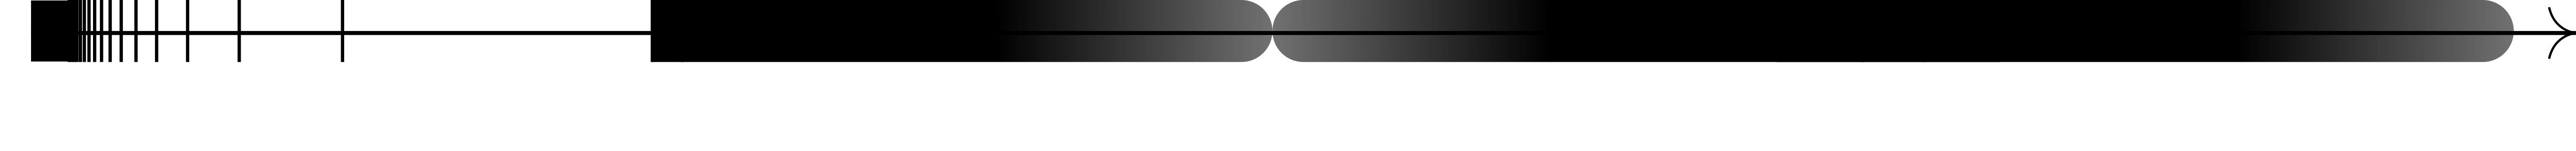
\includegraphics[width=0.8\textwidth]{set_a_.png}}}
    \only<6, 17>{\centering{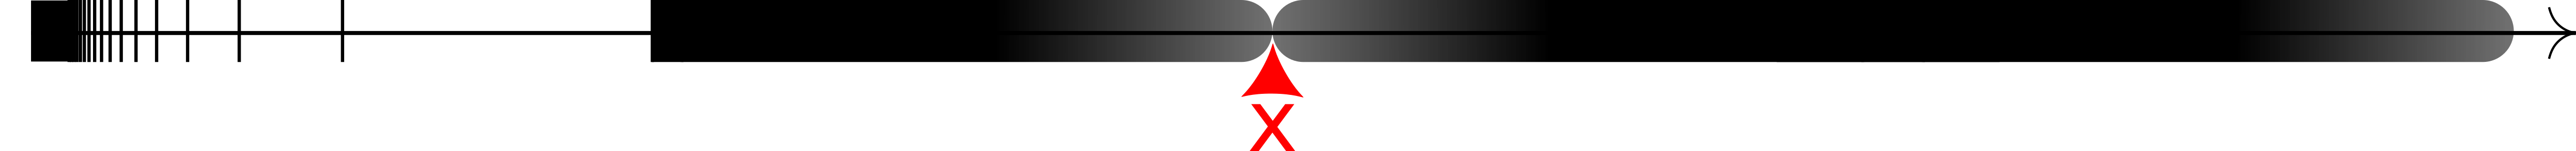
\includegraphics[width=0.8\textwidth]{set_a_2.png}}}
    \only<7, 18>{\centering{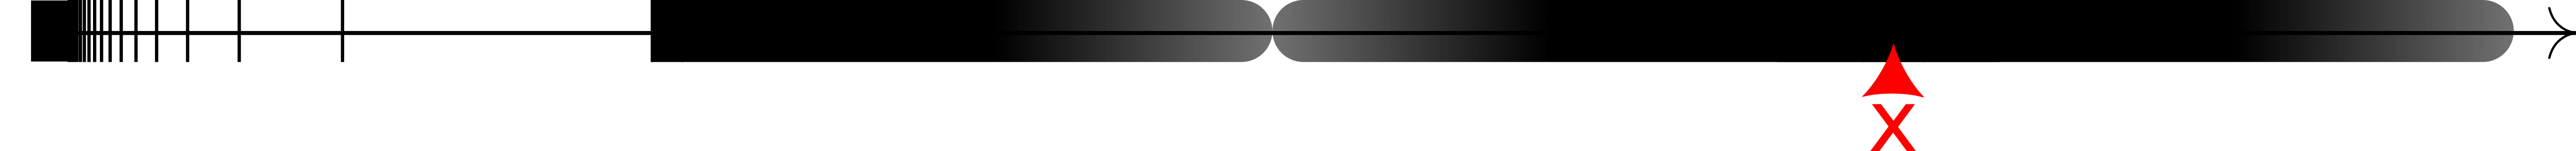
\includegraphics[width=0.8\textwidth]{set_a_3.png}}}
    \only<8>{\centering{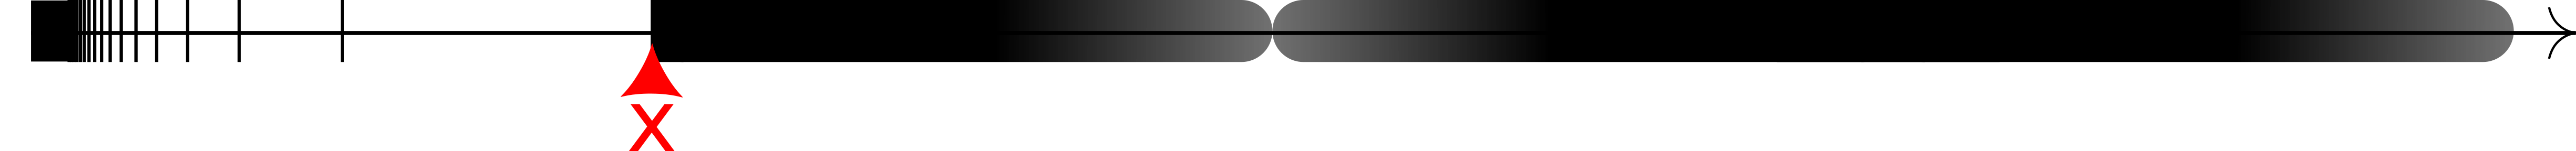
\includegraphics[width=0.8\textwidth]{set_a_1.png}}}
    \only<16>{\centering{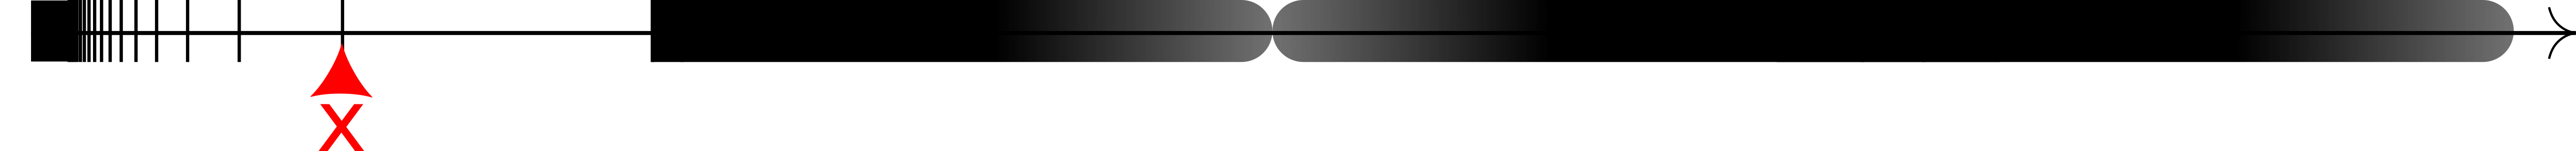
\includegraphics[width=0.8\textwidth]{set_a_1_2.png}}}
    \only<19, 22>{\centering{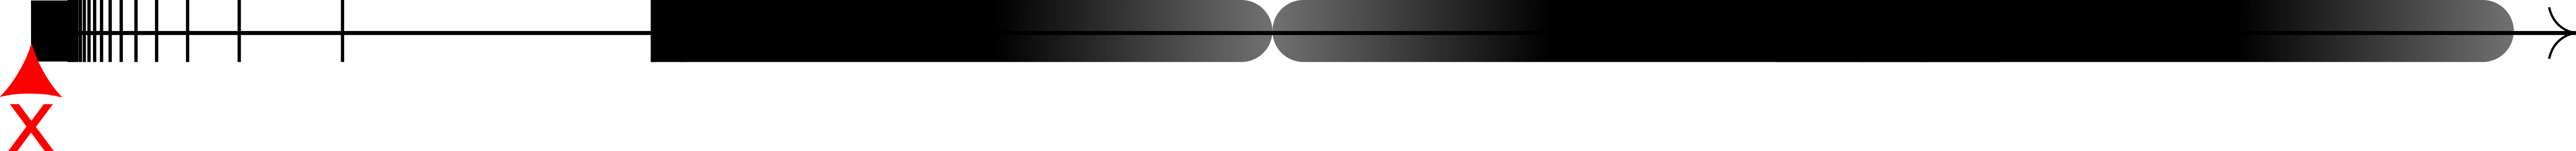
\includegraphics[width=0.8\textwidth]{set_a_0.png}}}
    \only<23>{\centering{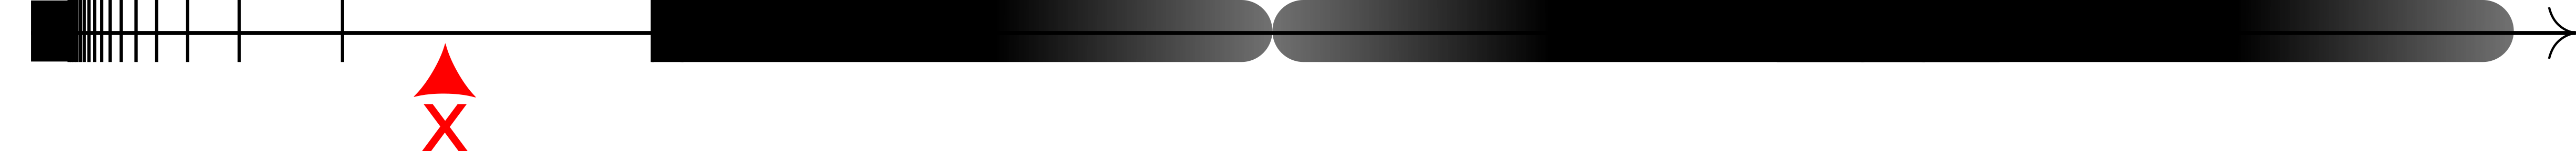
\includegraphics[width=0.8\textwidth]{set_a_2_3.png}}}
    %%% բովանդականություն
    \only<1>{
        \begin{block}{}
            \begin{itemize}
                \item ներքին
                \item կուտակման
                \item արտաքին
            \end{itemize}
        \end{block}
    }
    \only<2->{
        \begin{block}{Սահմանում}
            %%% ներքին կետի սահմանում
            \only<2-8>{$x$ կետը կոչվում է $A$ բազմության \alert<2>{ներքին կետ}, եթե $x$ կետի որոշակի շրջակայք ընկած է $A$ բազմության մեջ․
            \only<3, 4>{\[\exists \delta > 0 \; (x-\delta, x+\delta) \subset A\]}
            \only<5->{\[\exists \delta > 0 \; \alert<5>{U_\delta(x)} \subset A\]}}
            %%% կուտակման կեետի սահմանում
            \only<9-19>{\only<9->{$x$ կետը կոչվում է $A$ բազմություն \alert<9>{կուտակման կետ}, եթե \alert<11>{$x$ կետի ցանկացած շրջակայքում} գոյություն ունեն \alert<12>{$x$-ից տարբեր} $A$ բազմությանը պատկանող կետ․}
            \only<10-12>{\[\alert<11>{\forall \varepsilon > 0} \;  \exists y \in A \cap \alert<11>{U_\varepsilon(x)} \text{ և } \alert<12>{y \neq x}\]}
            \only<13-14>{\[\forall \varepsilon > 0 \;  \exists y \in A \cap U_\varepsilon(x) \backslash \{x\} \]}
            \only<15->{\[\forall \varepsilon > 0 \;  \exists y \in A \cap \alert<15>{\mathring{U}_\varepsilon(x)}\]}}
            %%% արտաքին կեետի սահմանում
            \only<20->{$x$ կետը կոչվում է $A$ բազմության \alert<20>{արտաքին կետ}, եթե $x$ կետի որոշակի շրջակայք $A$ բազմության հետ չի հատվում․
            \only<21->{\[\exists \delta > 0 \; U_\delta(x) \cap A = \emptyset\]}}

        \end{block}
    }
    \only<4, 14>{
        \begin{block}{Նշանակում}
            %%% միջակայքի նշանակում
            \only<4>{$x$ կետի $\delta$ միջակայքը նշանակվում է․
            \[U_\delta(x) := (x-\delta, x+\delta)\]}
            %%% ծակ միջակայքի նշանակում
            \only<14>{\[\mathring{U}_\delta(x) = U_\delta(x) \backslash \{x\} = (x-\delta, x) \cup (x, x+\delta)\]}
        \end{block}
    }
    \only<6-8, 16-19, 22-23>{
        \begin{exampleblock}{Օրինակ}
            %%% ներքին կետ
            \only<6>{$x = 2$ կատը $A$ բազմության ներքին կետ չէ։}
            \only<7>{$x = 3$ կատը $A$ բազմության ներքին կետ է։}
            \only<8>{$x = 1$ կատը $A$ բազմության ներքին կետ չէ։}
            %%% կուտակման կետ
            \only<16>{$x = \frac{1}{2}$ կատը $A$ բազմության կուտակման կետ չէ։}
            \only<17>{$x = 2$ կատը $A$ բազմության կուտակման կետ է։}
            \only<18>{$x = 3$ կատը $A$ բազմության կուտակման կետ է։}
            \only<19>{$x = 0$ կատը $A$ բազմության կուտակման կետ է։}
            %%% արտաքին կետ
            \only<22>{$x = 0$ կատը $A$ բազմության արտաքին կետ չէ։}
            \only<23>{$x = \frac{2}{3}$ կատը $A$ բազմության արտաքին կետ է։}
        \end{exampleblock}
    }
\end{frame}
\begin{frame}
    \frametitle{Ֆունկցիայի սահմանը $x$ կետում}
    %%% բովանդականություն
    \only<-36>{Դիցուք՝ $f: A \rightarrow \mathbb{R}$, իսկ \alert<4-5>{$x$-ը $A$ բազմության կուտակման կետ է}։}
    % \only<37->{$f(x) = \frac{\sin(x)}{x}$ ֆունկցիայի սահմանը $0$ կետում $1$ է։}
    \only<1>{
        \begin{block}{}
            \begin{itemize}
                \item սահմանը ըստ Հայնեի
                \item սահմանը ըստ Կոշիի
                \item ըստ Հայնեի $\Leftrightarrow$ ըստ Կոշիի
                \item օրիանկ $\frac{\sin(x)}{x}$ սահմանը $0$ կետում
            \end{itemize}
        \end{block}
    }
    \only<2-13>{
        \begin{block}{Սահմանումն ըստ \only<2-10>{Հայնեի}\only<11->{Կոշիի}}
            %%% ըստ Հայնեի
            \only<2-10>{Կասենք \alert<2>{$f$ ֆունկցիայի սահմաը $x$ կետում} $y$ է, եթե ցանկացած $a: \mathbb{N} \rightarrow A \cap \mathring{U}_\delta(x)$ $x$-ին զուգամիտող հաջորդականության համար, $b_n = f(a_n)$ զուգամիտում է $y$-ի․
            \only<3->{\[\lim_{n \rightarrow \infty}a_n = x \Rightarrow \lim_{n \rightarrow \infty}f(a_n) = y\]}}
            %%% Կոշիի
            \only<11->{Կասենք \alert<11>{$f$ ֆունկցիայի սահմաը $x$ կետում} $y$ է, եթե ցանկացած $U_\varepsilon(y)$ շրջակայքի համար կա այնպիսի $\mathring{U}_\delta(x)$ «շրջակայք», որի պատկերը ընկած է $U_\varepsilon(y)$ շրջակայքում․
            \only<12>{\[\forall U_\varepsilon(y) \; \exists \mathring{U}_\delta(x): \; f(\mathring{U}_\delta(x) \cap A) \subset U_\varepsilon(y)\]}}

        \end{block}
    }
    \only<4-10, 13>{
        \begin{alertblock}{} %%% դիտարկում
            %%% հաջորդականության կառուցում
            \only<4-10>{Կա այնպիսի $a: \mathbb{N} \rightarrow A \cap \mathring{U}_\delta(x)$, որ $\lim_{n \rightarrow \infty}a_n = x$:
            \only<5>{\[ a_1 = x_1 \alert{\in} A \cap \mathring{U}_1(x)\]}
            \only<6>{\[ a_1 = x_1 \in A \cap \mathring{U}_1(x) \qquad \delta_1 = \frac{|x - x_1|}{2} < \frac{1}{2}\]}
            \only<7>{\[ a_1 = x_1 \in A \cap \mathring{U}_1(x) \qquad 0 < \delta_1 = \frac{|x - x_1|}{2} < \frac{1}{2}\]}
            \only<8>{\[ a_2 = x_2 \in A \cap \mathring{U}_{\delta_1}(x) \qquad 0 < \delta_1 <\frac{1}{2} \qquad 0 < \delta_2 = \frac{|x - x_2|}{2} < \frac{1}{2^2}\]}
            \only<9>{\[ a_3 = x_3 \in A \cap \mathring{U}_{\delta_2}(x) \qquad 0 < \delta_2 <\frac{1}{2^2} \qquad 0 < \delta_3 = \frac{|x - x_3|}{2} < \frac{1}{2^3}\]}
            \only<10>{\[ a_n = x_n \in A \cap \mathring{U}_{\delta_{n-1}}(x) \qquad 0 < \delta_{n-1} <\frac{1}{2^{n-1}} \qquad 0 < \delta_n = \frac{|x - x_n|}{2} < \frac{1}{2^n}\]}}
            %%% Կոշիի պարզաբանում
            \only<13>{\[\forall \varepsilon > 0 \; \exists \delta_\varepsilon > 0: \; \forall x' \in A\backslash\{x\} \; |x - x'| < \delta \; |f(x') - y| < \varepsilon\]}
        \end{alertblock}
    }
    \only<14-36>{
        \begin{block}{Պնդում}
            $y$-ը $f$ ֆունկցիայի սահմանն է $x$ կետում ըստ Հայնեի այն և միայն այն դեպքում, երբ սահմանն է ըստ Կոշիի։
        \end{block}
    }
    \only<15-36>{
         \begin{alertblock}{Ապացույց  \only<17-26>{(Հայնե $\Rightarrow$ Կոշի)}\only<28->{(Կոշի $\Rightarrow$ Հայնե)}}
            %%% նկարագրություն
            \only<15-16, 27>{Պնդումն ապացուցելու համար, պետք ցույց տալ հետևյալ երկու դեպքերը․
            \begin{itemize}
                \item \alert<16>{$y$-ը սահմանն է ըստ Հայնեի $\Rightarrow$ $y$-ը սահմանն է ըստ Կոշիի},
                \item \alert<27>{$y$-ը սահմանն է ըստ Կոշիի $\Rightarrow$ $y$-ը սահմանն է ըստ Հայնեի}։
             \end{itemize}}
            %%% Հայնե ֊> Կոշի
            \only<17-26>{
                Ենթադրենք հակառակը․\\
                $y$-ը $f$ ֆունկցիայի սահմանն է $x$ կետում ըստ Հայնեի բայց \alert<17>{ոչ ըստ Կոշիի}։
                \only<18-19>{\[\exists U_\varepsilon(y)\; \forall \mathring{U}_\delta(x) \; \alert<19>{f(\mathring{U}_\delta(x) \cap A)\nsubset U_\varepsilon(y)}\]}
                \only<20>{\[\exists U_\varepsilon(y)\; \forall \mathring{U}_\delta(x) \; \exists y' \in f(\mathring{U}_\delta(x) \cap A): \; y' \notin U_\varepsilon(y)\]}
                \only<21-25>{\[\exists U_\varepsilon(y)\; \forall \mathring{U}_\delta(x) \; \exists x' \in \mathring{U}_\delta(x) \cap A: \;  f(x') = y' \notin U_\varepsilon(y)\]}
                \only<22>{\[0 < \delta_1 = 1 \qquad  a_1 = {x'}_1 \in A \cap \mathring{U}_{1}(x)  \qquad {y'}_1 = f(a_1) \notin U_\varepsilon(y)\]}
                \only<23>{\[0 < \delta_2 = \frac{|x - {x'}_1|}{2} < \frac{1}{2} \qquad  a_2 = {x'}_2 \in A \cap \mathring{U}_{\delta_2}(x)  \qquad {y'}_2 = f(a_2) \notin U_\varepsilon(y)\]}
                \only<24>{\[0 < \delta_3 = \frac{|x - {x'}_2|}{2} < \frac{1}{2^2} \qquad  a_3 = {x'}_3 \in A \cap \mathring{U}_{\delta_3}(x)  \qquad {y'}_3 = f(a_3) \notin U_\varepsilon(y)\]}
                \only<25>{\[0 < \delta_n = \frac{|x - {x'}_{n-1}|}{2} < \frac{1}{2^{n-1}} \qquad  a_n = {x'}_n \in A \cap \mathring{U}_{\delta_{n-1}}(x)  \qquad {y'}_n = f(a_n) \notin U_\varepsilon(y)\]}
                \only<26>{Ունենք, որ $\lim_{n \rightarrow \infty} a_n = x$, չնայած $b_n = f(a_n) \notin U_\varepsilon(y)$, որը հակասում է նրան, թե $\lim_{n \rightarrow \infty} b_n = y$:}
            }
            %%% Կոշի ֊> Հայնե
            \only<28-36>{
                Դիցուք՝\alert<34->{$a:\mathbb{N} \rightarrow A\backslash\{x\}$ հաջորդականությունը զուգամիտում է $x$-ի},\only<-30>{ այսինքն․}
                \only<29-30>{\[\lim_{n \rightarrow \infty}a_n = x\]}
                \only<30->{ցույց տանք, որ \alert<33>{$b_n = f(a_n)$} զուգամիտում է $y$-ի։}
                \only<31-35>{\[\alert<31, 35>{N_\varepsilon = ?} \; \forall n > N_\varepsilon\; |\alert<33>{b_n} - y| < \varepsilon\]}
                \only<36>{\[\alert<36>{N_\varepsilon = {N'}_{\delta_\varepsilon}} \; \forall n > N_\varepsilon\; |\alert<33>{b_n} - y| < \varepsilon\]}
                \only<32->{Քանի որ $y$-ը սահմանն է $f$ ֆունկցիայի $x$ կետում, \[|\alert<33>{f(a_n)} - y| < \varepsilon \text{, երբ } \alert<34->{0<|a_n - x|<\delta_\varepsilon}\]}
            }
            %%% Օրինակ
            \only<37>{
                \begin{exampleblock}
                    \[\lim_{n \rightarrow \infty} \frac{sin(x)}{x} = 1\]
                \end{exampleblock}
            }
        \end{alertblock}}
\end{frame}
\end{document}